\documentclass[11pt]{report}

%use European style
\usepackage[a4paper,left=2cm,right=2cm,top=2cm,bottom=2cm]{geometry}

%few useful packages ------------------------------------------------------------------
\usepackage{setspace}
\let\Tiny=\tiny %remove annoying warnings
\usepackage[english]{babel}
\usepackage[latin1]{inputenc}
\usepackage{amsmath}
\usepackage{amssymb}
\usepackage{amsthm}
\usepackage{amsfonts}
\usepackage{colortbl}
\usepackage{xcolor}
\usepackage{eurosym}
\usepackage{enumitem}
\usepackage{chngpage}
\usepackage{fancyhdr}
\usepackage{fancyvrb}
\usepackage{float}
\usepackage{framed}
\usepackage{multirow}
\usepackage{graphicx}
\graphicspath{ {./images/} }
\usepackage{geometry}
\usepackage{lipsum}
\usepackage{tabularx}
\usepackage[linktocpage]{hyperref}

%define environment for code
\definecolor{orangepse}{RGB}{240,139,39}
\definecolor{redpse}{RGB}{222,6,61}
\newcommand{\rpse}[1]{\textcolor{redpse}{#1}}
\definecolor{dkgreen}{rgb}{0,0.6,0}
\definecolor{gray}{rgb}{0.5,0.5,0.5}
\definecolor{mauve}{rgb}{0.58,0,0.82}

\usepackage{listings}
\lstset{frame=tblr,
	language=R,
	aboveskip=5mm,
	belowskip=5mm,
	showstringspaces=false,
	columns=flexible,
	basicstyle={\small\ttfamily},
	numbers=none,
	numberstyle=\tiny\color{gray},
	keywordstyle=\color{blue},
	commentstyle=\color{dkgreen},
	stringstyle=\color{mauve},
	breaklines=true,
	breakatwhitespace=true,
	tabsize=3
}
%---------------------------------------------------------------------------------------


% New Commands ----------------------------
\newcommand{\bb}{\bigbreak\noindent}

\makeatletter
\renewcommand\section{\leftskip 0pt\@startsection {section}{1}{\z@}%
	{-3.5ex \@plus -1ex \@minus -.2ex}%
	{2.3ex \@plus.2ex}%
	{\normalfont\Large\bfseries}}

\renewcommand\subsection{\leftskip 4ex\@startsection{subsection}{2}{\z@}%
	{-3.25ex\@plus -1ex \@minus -.2ex}%
	{1.5ex \@plus .2ex}%
	{\normalfont\large\bfseries}}

\renewcommand\subsubsection{\leftskip 14ex\@startsection{subsubsection}{3}{\z@}%
	{-3.25ex\@plus -1ex \@minus -.2ex}%
	{1.5ex \@plus .2ex}%
	{\normalfont\large\bfseries}}
\makeatother

%----------------------------------------------------------

\definecolor{titlepagecolor}{cmyk}{1,.60,0,.40}
\definecolor{namecolor}{cmyk}{1,.50,0,.10} 


\begin{document}
	\setcounter{page}{1}
	\begin{spacing}{1.5}
		
		% Table of Contents ----------------------------------
		\tableofcontents
		\setcounter{secnumdepth}{-2}
		\newpage
		
		% Start of Content ---------------------------------------------
		\chapter{General Notes:} 
		
		\chapter{Lecture 1: Measuring Aging}
		Defining ageing.
		\begin{itemize}
			\item Demographic Process
			\item Change in health
			\item Change in productivity
		\end{itemize}
		
		\section{Life Tables}
		\textbf{EXAM QUESTION EVERY YEAR:} What is the difference between period and cohort life tables
		
		\subsection{Observed data vs fictitious cohort}
		
		\begin{itemize}[leftmargin=10ex]
			\item  Period life table can be observed at each period, but does  not reflect mortality experience of a real cohort
			\item  Cohort life table can be observed once every individual of a cohort has died.
		\end{itemize}
		
		
		
		\section{Old Age Dependency Ratios}
		\[ \dfrac{Number \:\: of \:\: People \:\:Older \:\: than \:\:65}{Number \:\: of \:\: People \:\:between \:\: 15-65} \]
		\[ \dfrac{D_{65+}}{N_{15-64}} \]
		
	\section{Ageing by the Top}
	
		\subsection{From the bottom}
			Ageing driven by fertility decrease : reductions in number of youths or prime aged individuals
			\begin{itemize}[leftmargin=10ex]
				\item Historically decline in infant mortality led to increase in the share of the 60+
			\end{itemize}
			
		\subsection{From the Top}
		More recent realisation that recent ageing process is essentially ageing by the top
		\begin{itemize}[leftmargin=10ex]
			\item Recent gains in life expectancy come from gains at older ages
			\item Variety of experience at international level
		\end{itemize}
		
		
	\chapter{Institutional design of Pensions}
		\section{History Of Retirement}
			\subsection{Family Support}
			\subsection{Charity and Assistant}
			\subsection{Occupational Pensions}
			\subsection{Individual Savings}
			\subsection{Birth of the Welfare State: Bismark}
				\subsubsection{Work Related Accident Assurance}
				\subsubsection{Healthcare Insurance}
				Employers contributed one-third, the workers two-third\\
				``Sickness funds"", managed by workers' representatives
				
				\subsubsection{Old-age and disability insurance (1889)}
				Participation was mandatory (except for civil servants,covered by previous scheme) \\
				All workers concerned (not only industry workers)\\
				Contributory system funded by employee, employers and
				the State\\
				Pension age was set at 70. 
				\bb
				This was not about enjoying life after a career of hard work. This was strictly pragmatic. What do you expect from the Germans?
				
			\subsection{The UK and the Beverage Report}
			Unlike Bismark, the objective of the Beverage report was to lift all British out of poverty, but not to provide high replacement rates.
			\bb
			It was a comprehensive report that factored in all parts of living standards from cradle to grave. (Health system, Education, Housing, etc.)
			\bb
			An attack on the 5 evils:
			\begin{center}
				\textit{Want, Disease, Ignorance, Squalor, and Idleness.}
			\end{center}
			
		
		\section{Rationale for Public Intervention}
		
			\subsection{Market Failures}
				\subsubsection{Capital Markets}
				Large volatility in capital market returns\\
				Inflation could wipe out the value of someone's holdings very quickly in rare events.
				\bb
				Governments began to create index-linked bonds in an attempt to attenuate the effects of those events.
				
				
			\subsection{Myopia}
			People are often short sighted, and so they under-save for retirement
			
			\subsection{Samaritan's dilemma}
			If there is expectation that there will be assistance to the elderly poor (i.e., elderly cannot be left dying) Then some will under-save for retirement, expecting receiving welfare when poor
			\bb
			Governments will the intervene to attenuate the motivation to game the system.
			
			\subsection{Redistribution}
			Both within and between cohorts. (Some cohorts experience different shocks, large systems help smooth the effects of these)\\ 
			General objective to prevent poverty, especially of elderly individuals.
			
			\subsection{Efficiency and Administrative Costs}
			One of the benefits of compulsion is that no money is spent on selling insurance products by the state. But this harms competition and a uniform scheme might not accommodate heterogeneity in
			preferences (if too big).
			
		\section{Pension Design around the World}
		
			\subsection{Bismark vs Beveridge }
			
			\begin{figure}[h!]
				\centering
				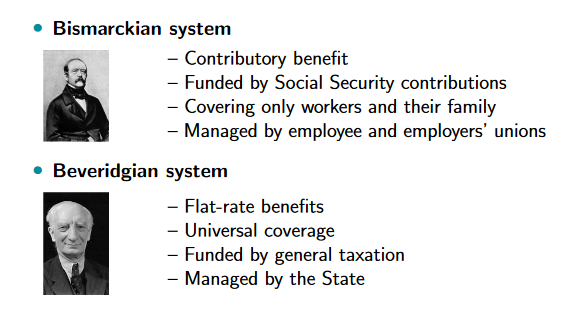
\includegraphics[width=0.7\linewidth]{screenshot001}
			\end{figure}
			
			Historically more complex\\
			Beveridge plan was in the form of a social insurance
			\begin{itemize}[leftmargin=10ex]
				\item Funded by National insurance contributions (NICs)
				\item Contributory benefits proportional to years of contribution
			\end{itemize}
			\bb
			Big difference : benefits expressed as absolute amount (not	as share of earnings). Evolution lead to marked difference with earnings-related schemes
		
		
		\section{Types of Pensions}
			\subsection{Public vs mandatory private vs voluntary private}
			\begin{itemize}[leftmargin=10ex]
				\item Mandatory systems can be public or private
				\item Mandate can be found with scheme monopoly or
				competition
				\item Public schemes can be run by the State or Social security
				administrations
			\end{itemize}
		
			\subsection{Funded vs unfunded vs mixed funding}
			Think of funding more as a spectrum with complete funding and unfunded being corner solutions.
			\begin{itemize}[leftmargin=10ex]
				\item  Funded : contributions invested in capital markets
				\item Unfunded or PAYGO : contributions directly used to
				finance current pensions
				\item Mixed funding : PAYGO with some reserves
			\end{itemize}
		
		
		
		
	\end{spacing}
\end{document}
